\documentclass[twoside]{book}

% Packages required by doxygen
\usepackage{fixltx2e}
\usepackage{calc}
\usepackage{doxygen}
\usepackage[export]{adjustbox} % also loads graphicx
\usepackage{graphicx}
\usepackage[utf8]{inputenc}
\usepackage{makeidx}
\usepackage{multicol}
\usepackage{multirow}
\PassOptionsToPackage{warn}{textcomp}
\usepackage{textcomp}
\usepackage[nointegrals]{wasysym}
\usepackage[table]{xcolor}

% Font selection
\usepackage[T1]{fontenc}
\usepackage[scaled=.90]{helvet}
\usepackage{courier}
\usepackage{amssymb}
\usepackage{sectsty}
\renewcommand{\familydefault}{\sfdefault}
\allsectionsfont{%
  \fontseries{bc}\selectfont%
  \color{darkgray}%
}
\renewcommand{\DoxyLabelFont}{%
  \fontseries{bc}\selectfont%
  \color{darkgray}%
}
\newcommand{\+}{\discretionary{\mbox{\scriptsize$\hookleftarrow$}}{}{}}

% Page & text layout
\usepackage{geometry}
\geometry{%
  a4paper,%
  top=2.5cm,%
  bottom=2.5cm,%
  left=2.5cm,%
  right=2.5cm%
}
\tolerance=750
\hfuzz=15pt
\hbadness=750
\setlength{\emergencystretch}{15pt}
\setlength{\parindent}{0cm}
\setlength{\parskip}{3ex plus 2ex minus 2ex}
\makeatletter
\renewcommand{\paragraph}{%
  \@startsection{paragraph}{4}{0ex}{-1.0ex}{1.0ex}{%
    \normalfont\normalsize\bfseries\SS@parafont%
  }%
}
\renewcommand{\subparagraph}{%
  \@startsection{subparagraph}{5}{0ex}{-1.0ex}{1.0ex}{%
    \normalfont\normalsize\bfseries\SS@subparafont%
  }%
}
\makeatother

% Headers & footers
\usepackage{fancyhdr}
\pagestyle{fancyplain}
\fancyhead[LE]{\fancyplain{}{\bfseries\thepage}}
\fancyhead[CE]{\fancyplain{}{}}
\fancyhead[RE]{\fancyplain{}{\bfseries\leftmark}}
\fancyhead[LO]{\fancyplain{}{\bfseries\rightmark}}
\fancyhead[CO]{\fancyplain{}{}}
\fancyhead[RO]{\fancyplain{}{\bfseries\thepage}}
\fancyfoot[LE]{\fancyplain{}{}}
\fancyfoot[CE]{\fancyplain{}{}}
\fancyfoot[RE]{\fancyplain{}{\bfseries\scriptsize Generated by Doxygen }}
\fancyfoot[LO]{\fancyplain{}{\bfseries\scriptsize Generated by Doxygen }}
\fancyfoot[CO]{\fancyplain{}{}}
\fancyfoot[RO]{\fancyplain{}{}}
\renewcommand{\footrulewidth}{0.4pt}
\renewcommand{\chaptermark}[1]{%
  \markboth{#1}{}%
}
\renewcommand{\sectionmark}[1]{%
  \markright{\thesection\ #1}%
}

% Indices & bibliography
\usepackage{natbib}
\usepackage[titles]{tocloft}
\setcounter{tocdepth}{3}
\setcounter{secnumdepth}{5}
\makeindex

% Hyperlinks (required, but should be loaded last)
\usepackage{ifpdf}
\ifpdf
  \usepackage[pdftex,pagebackref=true]{hyperref}
\else
  \usepackage[ps2pdf,pagebackref=true]{hyperref}
\fi
\hypersetup{%
  colorlinks=true,%
  linkcolor=blue,%
  citecolor=blue,%
  unicode%
}

% Custom commands
\newcommand{\clearemptydoublepage}{%
  \newpage{\pagestyle{empty}\cleardoublepage}%
}

\usepackage{caption}
\captionsetup{labelsep=space,justification=centering,font={bf},singlelinecheck=off,skip=4pt,position=top}

%===== C O N T E N T S =====

\begin{document}

% Titlepage & ToC
\hypersetup{pageanchor=false,
             bookmarksnumbered=true,
             pdfencoding=unicode
            }
\pagenumbering{roman}
\begin{titlepage}
\vspace*{7cm}
\begin{center}%
{\Large My Project }\\
\vspace*{1cm}
{\large Generated by Doxygen 1.8.11}\\
\end{center}
\end{titlepage}
\clearemptydoublepage
\tableofcontents
\clearemptydoublepage
\pagenumbering{arabic}
\hypersetup{pageanchor=true}

%--- Begin generated contents ---
\chapter{Hierarchical Index}
\section{Class Hierarchy}
This inheritance list is sorted roughly, but not completely, alphabetically\+:\begin{DoxyCompactList}
\item \contentsline{section}{Q\+Widget}{\pageref{classQWidget}}{}
\begin{DoxyCompactList}
\item \contentsline{section}{Login\+Window}{\pageref{classLoginWindow}}{}
\item \contentsline{section}{Pop\+Error}{\pageref{classPopError}}{}
\item \contentsline{section}{Registration\+Window}{\pageref{classRegistrationWindow}}{}
\end{DoxyCompactList}
\end{DoxyCompactList}

\chapter{Class Index}
\section{Class List}
Here are the classes, structs, unions and interfaces with brief descriptions\+:\begin{DoxyCompactList}
\item\contentsline{section}{\hyperlink{classLoginWindow}{Login\+Window} \\*Class which creates the G\+UI for login window }{\pageref{classLoginWindow}}{}
\item\contentsline{section}{\hyperlink{classRegistrationWindow}{Registration\+Window} }{\pageref{classRegistrationWindow}}{}
\end{DoxyCompactList}

\chapter{File Index}
\section{File List}
Here is a list of all documented files with brief descriptions\+:\begin{DoxyCompactList}
\item\contentsline{section}{\hyperlink{LoginWindow_8hpp}{Login\+Window.\+hpp} }{\pageref{LoginWindow_8hpp}}{}
\item\contentsline{section}{{\bfseries Registration\+Window.\+hpp} }{\pageref{RegistrationWindow_8hpp}}{}
\end{DoxyCompactList}

\chapter{Class Documentation}
\hypertarget{classLoginWindow}{}\section{Login\+Window Class Reference}
\label{classLoginWindow}\index{Login\+Window@{Login\+Window}}


\hyperlink{classLoginWindow}{Login\+Window} class which creates the G\+UI for login window.  




{\ttfamily \#include $<$Login\+Window.\+hpp$>$}



Inheritance diagram for Login\+Window\+:
% FIG 0


Collaboration diagram for Login\+Window\+:
% FIG 1
\subsection*{Public Types}
\begin{DoxyCompactItemize}
\item 
typedef std\+::string {\bfseries String}\hypertarget{classLoginWindow_a9d5191a38906ea9c5375c1029cfd9d4d}{}\label{classLoginWindow_a9d5191a38906ea9c5375c1029cfd9d4d}

\end{DoxyCompactItemize}
\subsection*{Public Slots}
\begin{DoxyCompactItemize}
\item 
void {\bfseries open\+Reg\+Win} ()\hypertarget{classLoginWindow_abe06ec97d678045c810e2ac6033ee9c0}{}\label{classLoginWindow_abe06ec97d678045c810e2ac6033ee9c0}

\item 
void {\bfseries check\+Login} (const Q\+String \&)\hypertarget{classLoginWindow_a01edb22f1bf6dfdf3bd0811f6c878330}{}\label{classLoginWindow_a01edb22f1bf6dfdf3bd0811f6c878330}

\item 
void \hyperlink{classLoginWindow_ad5a16b9244af77d36f98a4f48d3d423d}{check\+Password} (const Q\+String \&)
\item 
void {\bfseries send\+Login\+Req} ()\hypertarget{classLoginWindow_ac6dc94a63017e4e500b7ec0cbd4cac33}{}\label{classLoginWindow_ac6dc94a63017e4e500b7ec0cbd4cac33}

\end{DoxyCompactItemize}
\subsection*{Public Member Functions}
\begin{DoxyCompactItemize}
\item 
\hyperlink{classLoginWindow_ad3f4ec97bdb1fd55e3e6f6f25112f9d8}{Login\+Window} (Controller \&)
\begin{DoxyCompactList}\small\item\em \hyperlink{classLoginWindow}{Login\+Window} constructor for class \hyperlink{classLoginWindow}{Login\+Window} which creates G\+UI for login window. \end{DoxyCompactList}\item 
void \hyperlink{classLoginWindow_a1d429ebfb0f2ebb21591b209da5d4ecb}{close\+Reg\+Window} ()
\begin{DoxyCompactList}\small\item\em close\+Reg\+Window closing registration window \end{DoxyCompactList}\end{DoxyCompactItemize}


\subsection{Detailed Description}
\hyperlink{classLoginWindow}{Login\+Window} class which creates the G\+UI for login window. 

\subsection{Constructor \& Destructor Documentation}
\index{Login\+Window@{Login\+Window}!Login\+Window@{Login\+Window}}
\index{Login\+Window@{Login\+Window}!Login\+Window@{Login\+Window}}
\subsubsection[{\texorpdfstring{Login\+Window(\+Controller \&)}{LoginWindow(Controller &)}}]{\setlength{\rightskip}{0pt plus 5cm}Login\+Window\+::\+Login\+Window (
\begin{DoxyParamCaption}
\item[{Controller \&}]{c}
\end{DoxyParamCaption}
)}\hypertarget{classLoginWindow_ad3f4ec97bdb1fd55e3e6f6f25112f9d8}{}\label{classLoginWindow_ad3f4ec97bdb1fd55e3e6f6f25112f9d8}


\hyperlink{classLoginWindow}{Login\+Window} constructor for class \hyperlink{classLoginWindow}{Login\+Window} which creates G\+UI for login window. 


\begin{DoxyParams}{Parameters}
{\em is} & an initialized.... ?? \\
\hline
\end{DoxyParams}


\subsection{Member Function Documentation}
\index{Login\+Window@{Login\+Window}!check\+Password@{check\+Password}}
\index{check\+Password@{check\+Password}!Login\+Window@{Login\+Window}}
\subsubsection[{\texorpdfstring{check\+Password}{checkPassword}}]{\setlength{\rightskip}{0pt plus 5cm}void Login\+Window\+::check\+Password (
\begin{DoxyParamCaption}
\item[{const Q\+String \&}]{qs}
\end{DoxyParamCaption}
)\hspace{0.3cm}{\ttfamily [slot]}}\hypertarget{classLoginWindow_ad5a16b9244af77d36f98a4f48d3d423d}{}\label{classLoginWindow_ad5a16b9244af77d36f98a4f48d3d423d}
???????? \index{Login\+Window@{Login\+Window}!close\+Reg\+Window@{close\+Reg\+Window}}
\index{close\+Reg\+Window@{close\+Reg\+Window}!Login\+Window@{Login\+Window}}
\subsubsection[{\texorpdfstring{close\+Reg\+Window()}{closeRegWindow()}}]{\setlength{\rightskip}{0pt plus 5cm}void Login\+Window\+::close\+Reg\+Window (
\begin{DoxyParamCaption}
{}
\end{DoxyParamCaption}
)}\hypertarget{classLoginWindow_a1d429ebfb0f2ebb21591b209da5d4ecb}{}\label{classLoginWindow_a1d429ebfb0f2ebb21591b209da5d4ecb}


close\+Reg\+Window closing registration window 


\begin{DoxyParams}{Parameters}
{\em no} & parametrs \\
\hline
\end{DoxyParams}
\begin{DoxyReturn}{Returns}
void 
\end{DoxyReturn}


The documentation for this class was generated from the following files\+:\begin{DoxyCompactItemize}
\item 
\hyperlink{LoginWindow_8hpp}{Login\+Window.\+hpp}\item 
Login\+Window.\+cpp\end{DoxyCompactItemize}

\hypertarget{classPopError}{}\section{Pop\+Error Class Reference}
\label{classPopError}\index{Pop\+Error@{Pop\+Error}}


....  




{\ttfamily \#include $<$Pop\+Error.\+hpp$>$}



Inheritance diagram for Pop\+Error\+:
% FIG 0


Collaboration diagram for Pop\+Error\+:
% FIG 1
\subsection*{Public Types}
\begin{DoxyCompactItemize}
\item 
using {\bfseries String} = std\+::string\hypertarget{classPopError_a10f9b6cbf4bae9b9dd5226950c1a36be}{}\label{classPopError_a10f9b6cbf4bae9b9dd5226950c1a36be}

\end{DoxyCompactItemize}
\subsection*{Public Slots}
\begin{DoxyCompactItemize}
\item 
void {\bfseries set\+Text\+Slot} (const Q\+String \&)\hypertarget{classPopError_ad4e97cc2e18d85d68a8e2eab8c6c6261}{}\label{classPopError_ad4e97cc2e18d85d68a8e2eab8c6c6261}

\item 
void {\bfseries execute\+Slot} ()\hypertarget{classPopError_a083b9ed8c271233a26b0551bfb505393}{}\label{classPopError_a083b9ed8c271233a26b0551bfb505393}

\end{DoxyCompactItemize}
\subsection*{Signals}
\begin{DoxyCompactItemize}
\item 
void {\bfseries set\+Text\+Signal} (const Q\+String \&)\hypertarget{classPopError_af60b7e6052b6acdb4fb9d3b1897beff3}{}\label{classPopError_af60b7e6052b6acdb4fb9d3b1897beff3}

\item 
void {\bfseries execute\+Signal} ()\hypertarget{classPopError_a27399d28bccf522da4b51d5fbf230f23}{}\label{classPopError_a27399d28bccf522da4b51d5fbf230f23}

\end{DoxyCompactItemize}
\subsection*{Public Member Functions}
\begin{DoxyCompactItemize}
\item 
\hyperlink{classPopError_af8c8d37fd7a48ccf8d546a2a5cd90570}{Pop\+Error} ()
\begin{DoxyCompactList}\small\item\em .... \end{DoxyCompactList}\item 
void \hyperlink{classPopError_ae3536ead1943613df02fe7a3c1a04848}{handle\+Connection} ()
\begin{DoxyCompactList}\small\item\em .... \end{DoxyCompactList}\item 
void \hyperlink{classPopError_a1cd7be40b9010ac9ef46f560dacc91b9}{set\+Text} (const String \&)
\begin{DoxyCompactList}\small\item\em .... \end{DoxyCompactList}\item 
void \hyperlink{classPopError_a9a093bc81c3d1f2dccf37fa01186d9c9}{execute} ()
\begin{DoxyCompactList}\small\item\em ..... \end{DoxyCompactList}\end{DoxyCompactItemize}


\subsection{Detailed Description}
.... 

\subsection{Constructor \& Destructor Documentation}
\index{Pop\+Error@{Pop\+Error}!Pop\+Error@{Pop\+Error}}
\index{Pop\+Error@{Pop\+Error}!Pop\+Error@{Pop\+Error}}
\subsubsection[{\texorpdfstring{Pop\+Error()}{PopError()}}]{\setlength{\rightskip}{0pt plus 5cm}Pop\+Error\+::\+Pop\+Error (
\begin{DoxyParamCaption}
{}
\end{DoxyParamCaption}
)}\hypertarget{classPopError_af8c8d37fd7a48ccf8d546a2a5cd90570}{}\label{classPopError_af8c8d37fd7a48ccf8d546a2a5cd90570}


.... 


\begin{DoxyParams}{Parameters}
{\em ....} & \\
\hline
\end{DoxyParams}


\subsection{Member Function Documentation}
\index{Pop\+Error@{Pop\+Error}!execute@{execute}}
\index{execute@{execute}!Pop\+Error@{Pop\+Error}}
\subsubsection[{\texorpdfstring{execute()}{execute()}}]{\setlength{\rightskip}{0pt plus 5cm}void Pop\+Error\+::execute (
\begin{DoxyParamCaption}
{}
\end{DoxyParamCaption}
)}\hypertarget{classPopError_a9a093bc81c3d1f2dccf37fa01186d9c9}{}\label{classPopError_a9a093bc81c3d1f2dccf37fa01186d9c9}


..... 


\begin{DoxyParams}{Parameters}
{\em no} & parametrs \\
\hline
\end{DoxyParams}
\begin{DoxyReturn}{Returns}
void 
\end{DoxyReturn}
\index{Pop\+Error@{Pop\+Error}!handle\+Connection@{handle\+Connection}}
\index{handle\+Connection@{handle\+Connection}!Pop\+Error@{Pop\+Error}}
\subsubsection[{\texorpdfstring{handle\+Connection()}{handleConnection()}}]{\setlength{\rightskip}{0pt plus 5cm}void Pop\+Error\+::handle\+Connection (
\begin{DoxyParamCaption}
{}
\end{DoxyParamCaption}
)}\hypertarget{classPopError_ae3536ead1943613df02fe7a3c1a04848}{}\label{classPopError_ae3536ead1943613df02fe7a3c1a04848}


.... 


\begin{DoxyParams}{Parameters}
{\em ...} & \\
\hline
\end{DoxyParams}
\begin{DoxyReturn}{Returns}
void 
\end{DoxyReturn}
\index{Pop\+Error@{Pop\+Error}!set\+Text@{set\+Text}}
\index{set\+Text@{set\+Text}!Pop\+Error@{Pop\+Error}}
\subsubsection[{\texorpdfstring{set\+Text(const String \&)}{setText(const String &)}}]{\setlength{\rightskip}{0pt plus 5cm}void Pop\+Error\+::set\+Text (
\begin{DoxyParamCaption}
\item[{const String \&}]{s}
\end{DoxyParamCaption}
)}\hypertarget{classPopError_a1cd7be40b9010ac9ef46f560dacc91b9}{}\label{classPopError_a1cd7be40b9010ac9ef46f560dacc91b9}


.... 


\begin{DoxyParams}{Parameters}
{\em ....} & \\
\hline
\end{DoxyParams}
\begin{DoxyReturn}{Returns}
void 
\end{DoxyReturn}


The documentation for this class was generated from the following files\+:\begin{DoxyCompactItemize}
\item 
gui/\hyperlink{PopError_8hpp}{Pop\+Error.\+hpp}\item 
gui/Pop\+Error.\+cpp\end{DoxyCompactItemize}

\hypertarget{classQWidget}{}\section{Q\+Widget Class Reference}
\label{classQWidget}\index{Q\+Widget@{Q\+Widget}}


Inheritance diagram for Q\+Widget\+:
\nopagebreak
\begin{figure}[H]
\begin{center}
\leavevmode
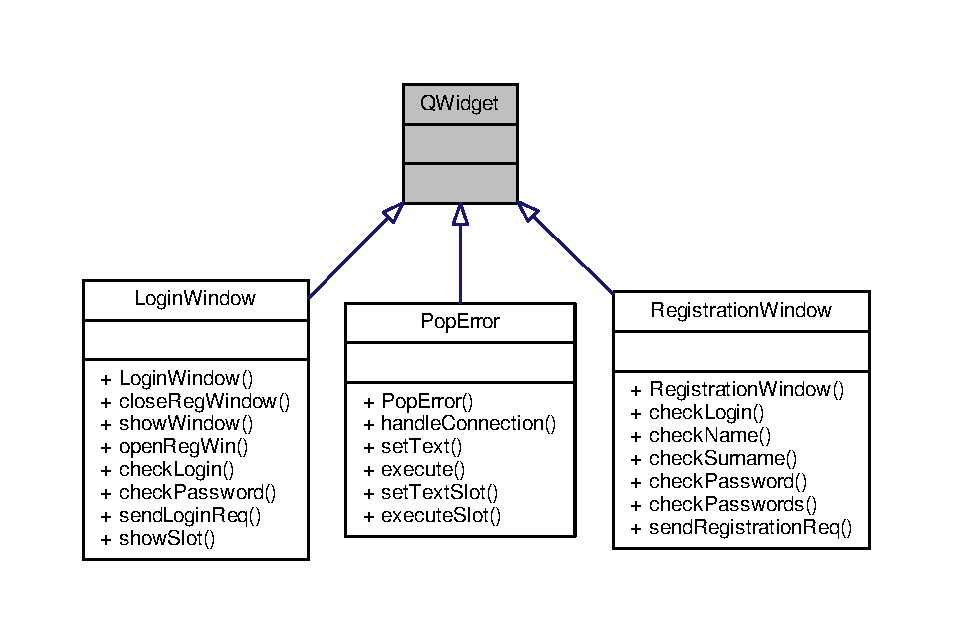
\includegraphics[width=350pt]{classQWidget__inherit__graph}
\end{center}
\end{figure}


Collaboration diagram for Q\+Widget\+:
\nopagebreak
\begin{figure}[H]
\begin{center}
\leavevmode
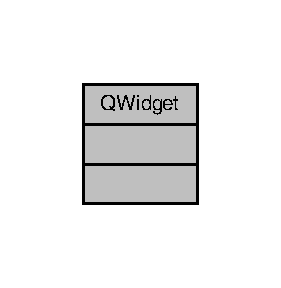
\includegraphics[width=135pt]{classQWidget__coll__graph}
\end{center}
\end{figure}


The documentation for this class was generated from the following file\+:\begin{DoxyCompactItemize}
\item 
\hyperlink{LoginWindow_8hpp}{Login\+Window.\+hpp}\end{DoxyCompactItemize}

\hypertarget{classRegistrationWindow}{}\section{Registration\+Window Class Reference}
\label{classRegistrationWindow}\index{Registration\+Window@{Registration\+Window}}


\hyperlink{classRegistrationWindow}{Registration\+Window} class which creates the G\+UI for login window.  




{\ttfamily \#include $<$Registration\+Window.\+hpp$>$}



Inheritance diagram for Registration\+Window\+:
\nopagebreak
\begin{figure}[H]
\begin{center}
\leavevmode
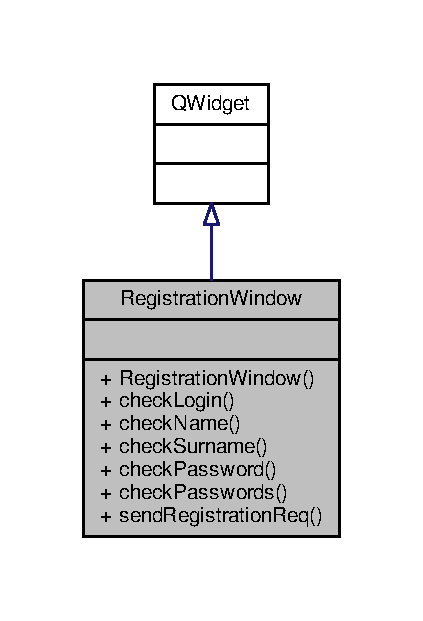
\includegraphics[width=203pt]{classRegistrationWindow__inherit__graph}
\end{center}
\end{figure}


Collaboration diagram for Registration\+Window\+:
\nopagebreak
\begin{figure}[H]
\begin{center}
\leavevmode
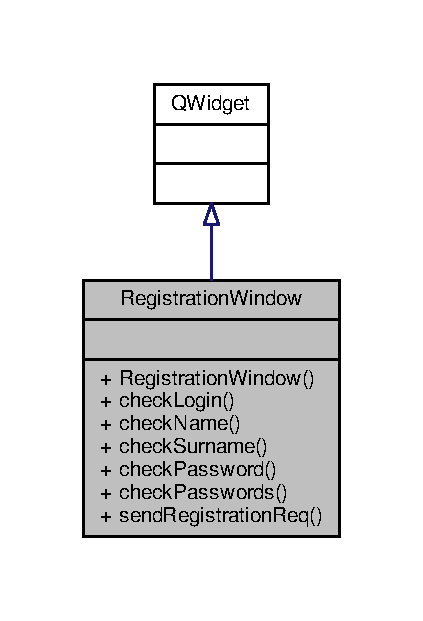
\includegraphics[width=203pt]{classRegistrationWindow__coll__graph}
\end{center}
\end{figure}
\subsection*{Public Types}
\begin{DoxyCompactItemize}
\item 
using \hyperlink{classRegistrationWindow_af737e72502243796bee87789c8b5b9ea}{String} = std\+::string
\end{DoxyCompactItemize}
\subsection*{Public Slots}
\begin{DoxyCompactItemize}
\item 
void \hyperlink{classRegistrationWindow_a054fcf4544f917e106aa6760f720d7b2}{check\+Login} (const Q\+String \&)
\item 
void \hyperlink{classRegistrationWindow_a26d58595ac8df47a0456878a80c45ffc}{check\+Name} (const Q\+String \&)
\item 
void \hyperlink{classRegistrationWindow_a6fc9f673b5e1d2fd15c9e12bfc0174b2}{check\+Surname} (const Q\+String \&)
\item 
void \hyperlink{classRegistrationWindow_a761ec197a38b335aaa5db06287361849}{check\+Password} (const Q\+String \&)
\item 
void \hyperlink{classRegistrationWindow_a6c3761195b00134d3ef4decf91ea76e7}{check\+Passwords} (const Q\+String \&)
\item 
void \hyperlink{classRegistrationWindow_a4344e4dafa6ab47e564c243b20a0c7a4}{send\+Registration\+Req} ()
\end{DoxyCompactItemize}
\subsection*{Public Member Functions}
\begin{DoxyCompactItemize}
\item 
\hyperlink{classRegistrationWindow_ac8876ad29199208fc8b8bd25863c9318}{Registration\+Window} (Controller \&)
\begin{DoxyCompactList}\small\item\em \hyperlink{classRegistrationWindow}{Registration\+Window} constructor for class \hyperlink{classRegistrationWindow}{Registration\+Window} which creates G\+UI for registration window. \end{DoxyCompactList}\end{DoxyCompactItemize}


\subsection{Detailed Description}
\hyperlink{classRegistrationWindow}{Registration\+Window} class which creates the G\+UI for login window. 

\subsection{Member Typedef Documentation}
\index{Registration\+Window@{Registration\+Window}!String@{String}}
\index{String@{String}!Registration\+Window@{Registration\+Window}}
\subsubsection[{\texorpdfstring{String}{String}}]{\setlength{\rightskip}{0pt plus 5cm}using {\bf Registration\+Window\+::\+String} =  std\+::string}\hypertarget{classRegistrationWindow_af737e72502243796bee87789c8b5b9ea}{}\label{classRegistrationWindow_af737e72502243796bee87789c8b5b9ea}


\subsection{Constructor \& Destructor Documentation}
\index{Registration\+Window@{Registration\+Window}!Registration\+Window@{Registration\+Window}}
\index{Registration\+Window@{Registration\+Window}!Registration\+Window@{Registration\+Window}}
\subsubsection[{\texorpdfstring{Registration\+Window(\+Controller \&)}{RegistrationWindow(Controller &)}}]{\setlength{\rightskip}{0pt plus 5cm}Registration\+Window\+::\+Registration\+Window (
\begin{DoxyParamCaption}
\item[{Controller \&}]{c}
\end{DoxyParamCaption}
)}\hypertarget{classRegistrationWindow_ac8876ad29199208fc8b8bd25863c9318}{}\label{classRegistrationWindow_ac8876ad29199208fc8b8bd25863c9318}


\hyperlink{classRegistrationWindow}{Registration\+Window} constructor for class \hyperlink{classRegistrationWindow}{Registration\+Window} which creates G\+UI for registration window. 


\begin{DoxyParams}{Parameters}
{\em is} & an initialized......??? \\
\hline
\end{DoxyParams}


\subsection{Member Function Documentation}
\index{Registration\+Window@{Registration\+Window}!check\+Login@{check\+Login}}
\index{check\+Login@{check\+Login}!Registration\+Window@{Registration\+Window}}
\subsubsection[{\texorpdfstring{check\+Login}{checkLogin}}]{\setlength{\rightskip}{0pt plus 5cm}void Registration\+Window\+::check\+Login (
\begin{DoxyParamCaption}
\item[{const Q\+String \&}]{qs}
\end{DoxyParamCaption}
)\hspace{0.3cm}{\ttfamily [slot]}}\hypertarget{classRegistrationWindow_a054fcf4544f917e106aa6760f720d7b2}{}\label{classRegistrationWindow_a054fcf4544f917e106aa6760f720d7b2}
\index{Registration\+Window@{Registration\+Window}!check\+Name@{check\+Name}}
\index{check\+Name@{check\+Name}!Registration\+Window@{Registration\+Window}}
\subsubsection[{\texorpdfstring{check\+Name}{checkName}}]{\setlength{\rightskip}{0pt plus 5cm}void Registration\+Window\+::check\+Name (
\begin{DoxyParamCaption}
\item[{const Q\+String \&}]{qs}
\end{DoxyParamCaption}
)\hspace{0.3cm}{\ttfamily [slot]}}\hypertarget{classRegistrationWindow_a26d58595ac8df47a0456878a80c45ffc}{}\label{classRegistrationWindow_a26d58595ac8df47a0456878a80c45ffc}
\index{Registration\+Window@{Registration\+Window}!check\+Password@{check\+Password}}
\index{check\+Password@{check\+Password}!Registration\+Window@{Registration\+Window}}
\subsubsection[{\texorpdfstring{check\+Password}{checkPassword}}]{\setlength{\rightskip}{0pt plus 5cm}void Registration\+Window\+::check\+Password (
\begin{DoxyParamCaption}
\item[{const Q\+String \&}]{qs}
\end{DoxyParamCaption}
)\hspace{0.3cm}{\ttfamily [slot]}}\hypertarget{classRegistrationWindow_a761ec197a38b335aaa5db06287361849}{}\label{classRegistrationWindow_a761ec197a38b335aaa5db06287361849}
\index{Registration\+Window@{Registration\+Window}!check\+Passwords@{check\+Passwords}}
\index{check\+Passwords@{check\+Passwords}!Registration\+Window@{Registration\+Window}}
\subsubsection[{\texorpdfstring{check\+Passwords}{checkPasswords}}]{\setlength{\rightskip}{0pt plus 5cm}void Registration\+Window\+::check\+Passwords (
\begin{DoxyParamCaption}
\item[{const Q\+String \&}]{qs}
\end{DoxyParamCaption}
)\hspace{0.3cm}{\ttfamily [slot]}}\hypertarget{classRegistrationWindow_a6c3761195b00134d3ef4decf91ea76e7}{}\label{classRegistrationWindow_a6c3761195b00134d3ef4decf91ea76e7}
\index{Registration\+Window@{Registration\+Window}!check\+Surname@{check\+Surname}}
\index{check\+Surname@{check\+Surname}!Registration\+Window@{Registration\+Window}}
\subsubsection[{\texorpdfstring{check\+Surname}{checkSurname}}]{\setlength{\rightskip}{0pt plus 5cm}void Registration\+Window\+::check\+Surname (
\begin{DoxyParamCaption}
\item[{const Q\+String \&}]{qs}
\end{DoxyParamCaption}
)\hspace{0.3cm}{\ttfamily [slot]}}\hypertarget{classRegistrationWindow_a6fc9f673b5e1d2fd15c9e12bfc0174b2}{}\label{classRegistrationWindow_a6fc9f673b5e1d2fd15c9e12bfc0174b2}
\index{Registration\+Window@{Registration\+Window}!send\+Registration\+Req@{send\+Registration\+Req}}
\index{send\+Registration\+Req@{send\+Registration\+Req}!Registration\+Window@{Registration\+Window}}
\subsubsection[{\texorpdfstring{send\+Registration\+Req}{sendRegistrationReq}}]{\setlength{\rightskip}{0pt plus 5cm}void Registration\+Window\+::send\+Registration\+Req (
\begin{DoxyParamCaption}
{}
\end{DoxyParamCaption}
)\hspace{0.3cm}{\ttfamily [slot]}}\hypertarget{classRegistrationWindow_a4344e4dafa6ab47e564c243b20a0c7a4}{}\label{classRegistrationWindow_a4344e4dafa6ab47e564c243b20a0c7a4}


The documentation for this class was generated from the following files\+:\begin{DoxyCompactItemize}
\item 
\hyperlink{RegistrationWindow_8hpp}{Registration\+Window.\+hpp}\item 
\hyperlink{RegistrationWindow_8cpp}{Registration\+Window.\+cpp}\end{DoxyCompactItemize}

\chapter{File Documentation}
\hypertarget{LoginWindow_8cpp}{}\section{Login\+Window.\+cpp File Reference}
\label{LoginWindow_8cpp}\index{Login\+Window.\+cpp@{Login\+Window.\+cpp}}
{\ttfamily \#include $<$iostream$>$}\\*
{\ttfamily \#include $<$Q\+Label$>$}\\*
{\ttfamily \#include $<$Q\+Palette$>$}\\*
{\ttfamily \#include \char`\"{}Login\+Window.\+hpp\char`\"{}}\\*
{\ttfamily \#include \char`\"{}../core/\+Validation\+Info.\+hpp\char`\"{}}\\*
Include dependency graph for Login\+Window.\+cpp\+:
\nopagebreak
\begin{figure}[H]
\begin{center}
\leavevmode
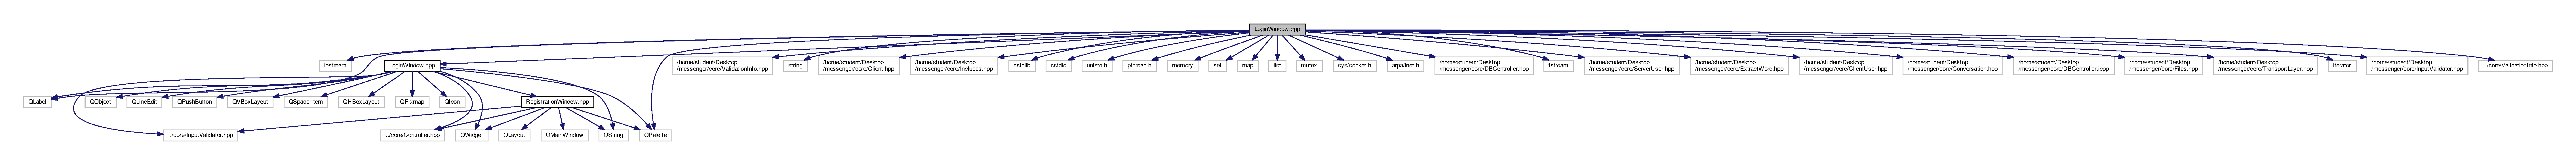
\includegraphics[width=350pt]{LoginWindow_8cpp__incl}
\end{center}
\end{figure}

\hypertarget{LoginWindow_8hpp}{}\section{Login\+Window.\+hpp File Reference}
\label{LoginWindow_8hpp}\index{Login\+Window.\+hpp@{Login\+Window.\+hpp}}


\hyperlink{LoginWindow_8hpp}{Login\+Window.\+hpp} creating a G\+UI for login window and connection for checking the login password.  


{\ttfamily \#include $<$Q\+Object$>$}\\*
{\ttfamily \#include $<$Q\+Widget$>$}\\*
{\ttfamily \#include $<$Q\+Line\+Edit$>$}\\*
{\ttfamily \#include $<$Q\+Push\+Button$>$}\\*
{\ttfamily \#include $<$Q\+V\+Box\+Layout$>$}\\*
{\ttfamily \#include $<$Q\+Spacer\+Item$>$}\\*
{\ttfamily \#include $<$Q\+H\+Box\+Layout$>$}\\*
{\ttfamily \#include $<$Q\+Label$>$}\\*
{\ttfamily \#include $<$Q\+Pixmap$>$}\\*
{\ttfamily \#include $<$Q\+Palette$>$}\\*
{\ttfamily \#include $<$Q\+Icon$>$}\\*
{\ttfamily \#include $<$Q\+String$>$}\\*
{\ttfamily \#include \char`\"{}Registration\+Window.\+hpp\char`\"{}}\\*
{\ttfamily \#include \char`\"{}../core/\+Input\+Validator.\+hpp\char`\"{}}\\*
{\ttfamily \#include \char`\"{}../core/\+Controller.\+hpp\char`\"{}}\\*
Include dependency graph for Login\+Window.\+hpp\+:

\hypertarget{Main_8cpp}{}\section{Main.\+cpp File Reference}
\label{Main_8cpp}\index{Main.\+cpp@{Main.\+cpp}}
{\ttfamily \#include \char`\"{}../core/\+Client.\+hpp\char`\"{}}\\*
{\ttfamily \#include \char`\"{}../core/\+Controller.\+hpp\char`\"{}}\\*
{\ttfamily \#include \char`\"{}./\+Main\+Window/\+Main\+Window.\+hpp\char`\"{}}\\*
{\ttfamily \#include $<$Q\+Application$>$}\\*
Include dependency graph for Main.\+cpp\+:
\nopagebreak
\begin{figure}[H]
\begin{center}
\leavevmode
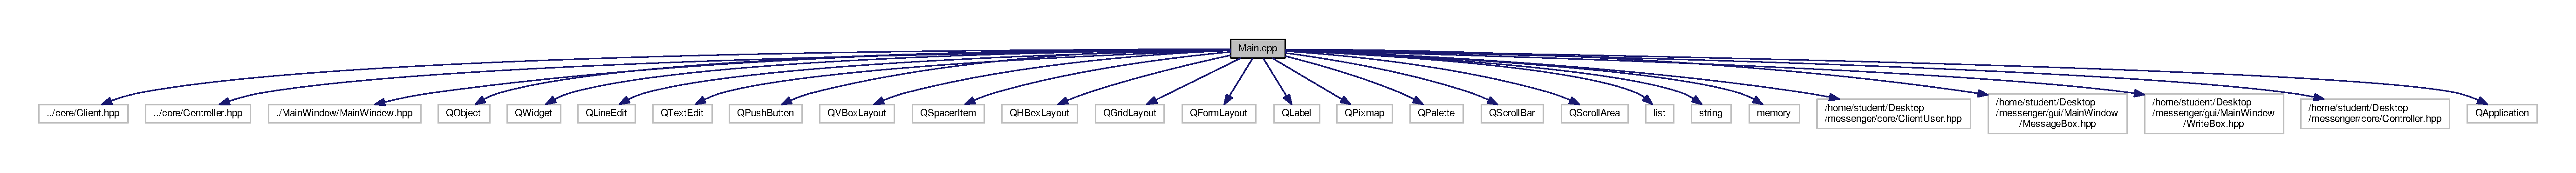
\includegraphics[width=350pt]{Main_8cpp__incl}
\end{center}
\end{figure}
\subsection*{Functions}
\begin{DoxyCompactItemize}
\item 
int \hyperlink{Main_8cpp_a0ddf1224851353fc92bfbff6f499fa97}{main} (int argc, char $\ast$argv\mbox{[}$\,$\mbox{]})
\end{DoxyCompactItemize}


\subsection{Function Documentation}
\index{Main.\+cpp@{Main.\+cpp}!main@{main}}
\index{main@{main}!Main.\+cpp@{Main.\+cpp}}
\subsubsection[{\texorpdfstring{main(int argc, char $\ast$argv[])}{main(int argc, char *argv[])}}]{\setlength{\rightskip}{0pt plus 5cm}int main (
\begin{DoxyParamCaption}
\item[{int}]{argc, }
\item[{char $\ast$}]{argv\mbox{[}$\,$\mbox{]}}
\end{DoxyParamCaption}
)}\hypertarget{Main_8cpp_a0ddf1224851353fc92bfbff6f499fa97}{}\label{Main_8cpp_a0ddf1224851353fc92bfbff6f499fa97}

\hypertarget{moc__Avatar_8cpp}{}\section{moc\+\_\+\+Avatar.\+cpp File Reference}
\label{moc__Avatar_8cpp}\index{moc\+\_\+\+Avatar.\+cpp@{moc\+\_\+\+Avatar.\+cpp}}
{\ttfamily \#include \char`\"{}Main\+Window/\+Avatar.\+hpp\char`\"{}}\\*
Include dependency graph for moc\+\_\+\+Avatar.\+cpp\+:
\nopagebreak
\begin{figure}[H]
\begin{center}
\leavevmode
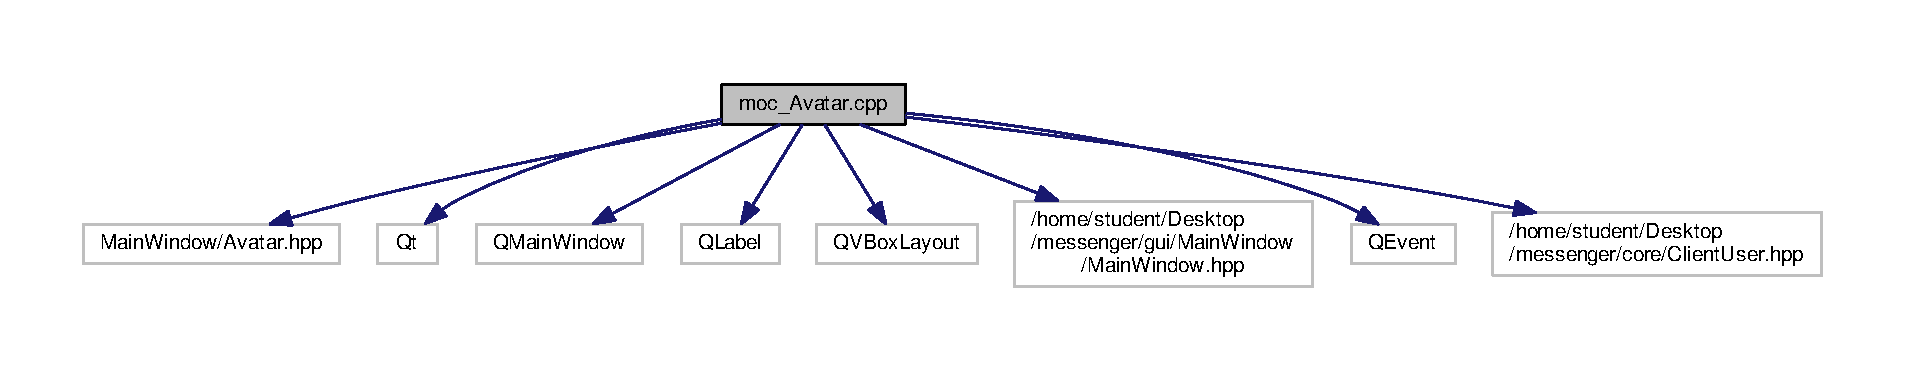
\includegraphics[width=350pt]{moc__Avatar_8cpp__incl}
\end{center}
\end{figure}

\hypertarget{moc__LoginWindow_8cpp}{}\section{moc\+\_\+\+Login\+Window.\+cpp File Reference}
\label{moc__LoginWindow_8cpp}\index{moc\+\_\+\+Login\+Window.\+cpp@{moc\+\_\+\+Login\+Window.\+cpp}}
{\ttfamily \#include \char`\"{}Login\+Window.\+hpp\char`\"{}}\\*
Include dependency graph for moc\+\_\+\+Login\+Window.\+cpp\+:
\nopagebreak
\begin{figure}[H]
\begin{center}
\leavevmode
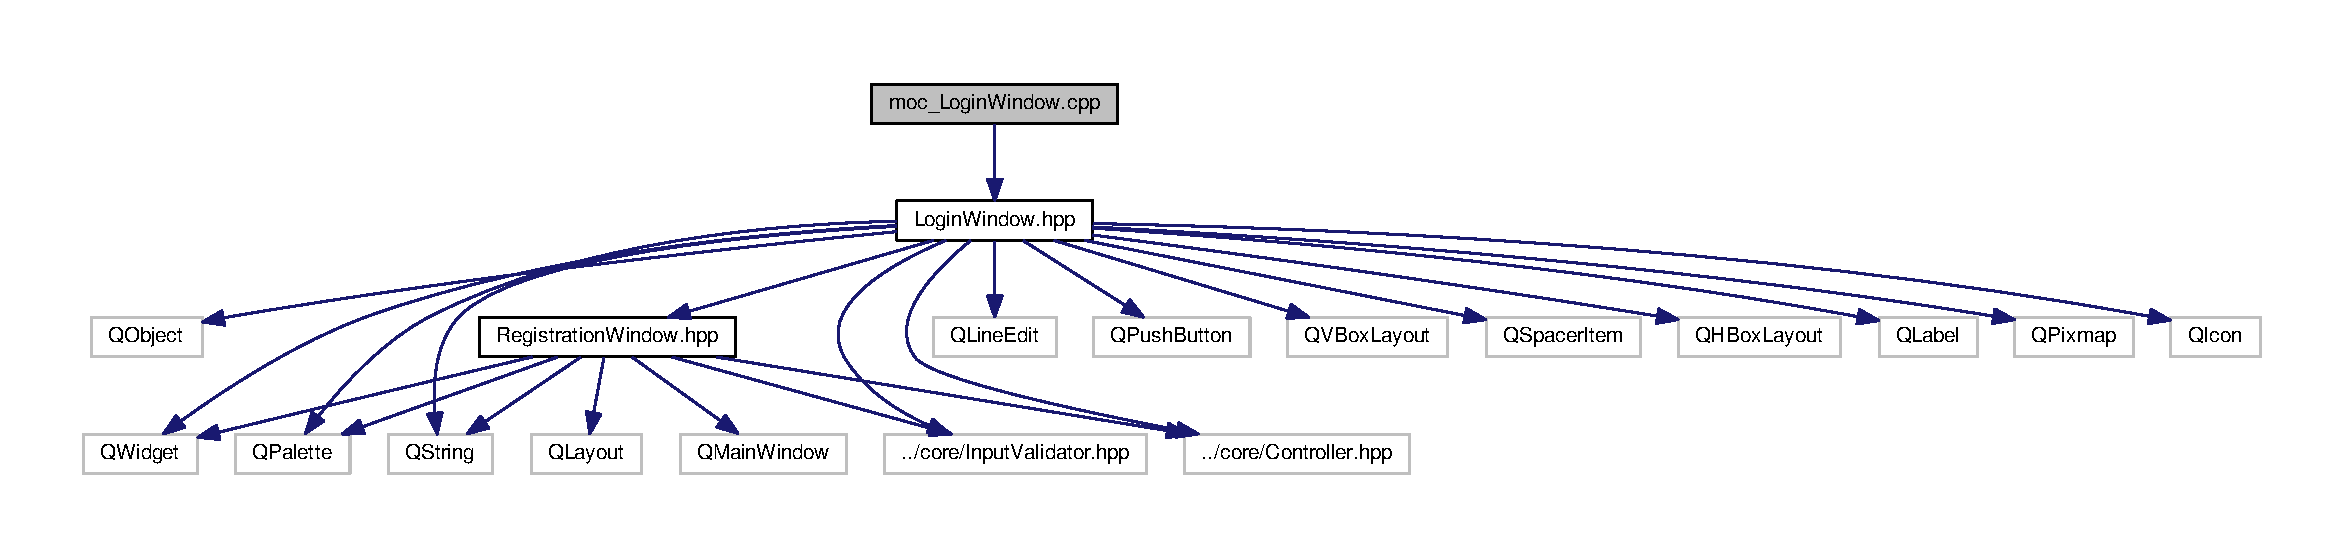
\includegraphics[width=350pt]{moc__LoginWindow_8cpp__incl}
\end{center}
\end{figure}

\hypertarget{moc__MainWindow_8cpp}{}\section{moc\+\_\+\+Main\+Window.\+cpp File Reference}
\label{moc__MainWindow_8cpp}\index{moc\+\_\+\+Main\+Window.\+cpp@{moc\+\_\+\+Main\+Window.\+cpp}}
{\ttfamily \#include \char`\"{}Main\+Window/\+Main\+Window.\+hpp\char`\"{}}\\*
Include dependency graph for moc\+\_\+\+Main\+Window.\+cpp\+:
\nopagebreak
\begin{figure}[H]
\begin{center}
\leavevmode
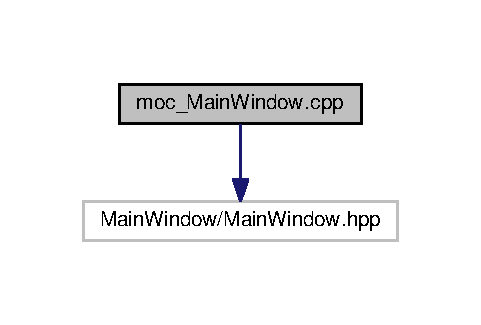
\includegraphics[width=231pt]{moc__MainWindow_8cpp__incl}
\end{center}
\end{figure}

\hypertarget{moc__PopError_8cpp}{}\section{moc\+\_\+\+Pop\+Error.\+cpp File Reference}
\label{moc__PopError_8cpp}\index{moc\+\_\+\+Pop\+Error.\+cpp@{moc\+\_\+\+Pop\+Error.\+cpp}}
{\ttfamily \#include \char`\"{}Pop\+Error.\+hpp\char`\"{}}\\*
Include dependency graph for moc\+\_\+\+Pop\+Error.\+cpp\+:
\nopagebreak
\begin{figure}[H]
\begin{center}
\leavevmode
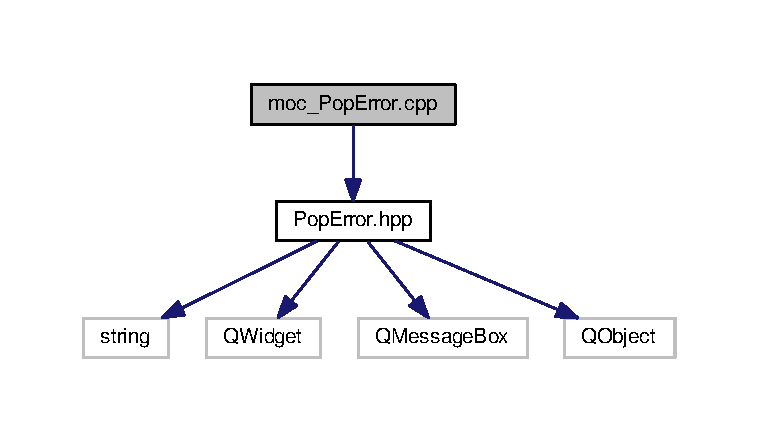
\includegraphics[width=350pt]{moc__PopError_8cpp__incl}
\end{center}
\end{figure}

\hypertarget{moc__RegistrationWindow_8cpp}{}\section{moc\+\_\+\+Registration\+Window.\+cpp File Reference}
\label{moc__RegistrationWindow_8cpp}\index{moc\+\_\+\+Registration\+Window.\+cpp@{moc\+\_\+\+Registration\+Window.\+cpp}}
{\ttfamily \#include \char`\"{}Registration\+Window.\+hpp\char`\"{}}\\*
Include dependency graph for moc\+\_\+\+Registration\+Window.\+cpp\+:
\nopagebreak
\begin{figure}[H]
\begin{center}
\leavevmode
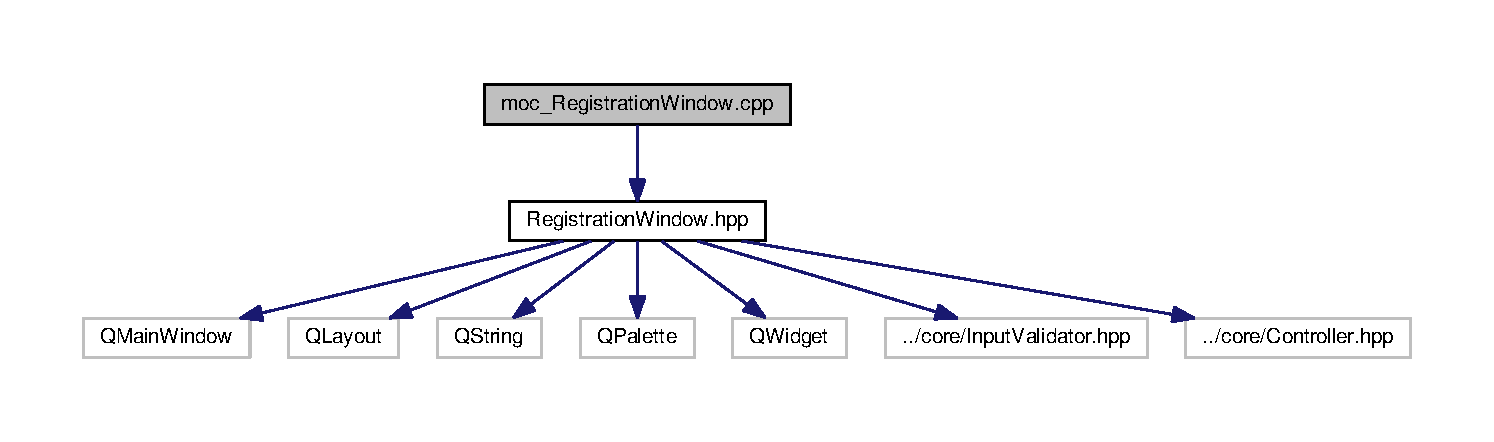
\includegraphics[width=350pt]{moc__RegistrationWindow_8cpp__incl}
\end{center}
\end{figure}

\hypertarget{moc__WriteBox_8cpp}{}\section{moc\+\_\+\+Write\+Box.\+cpp File Reference}
\label{moc__WriteBox_8cpp}\index{moc\+\_\+\+Write\+Box.\+cpp@{moc\+\_\+\+Write\+Box.\+cpp}}
{\ttfamily \#include \char`\"{}Main\+Window/\+Write\+Box.\+hpp\char`\"{}}\\*
Include dependency graph for moc\+\_\+\+Write\+Box.\+cpp\+:
\nopagebreak
\begin{figure}[H]
\begin{center}
\leavevmode
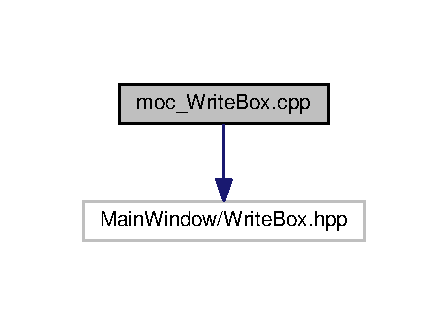
\includegraphics[width=215pt]{moc__WriteBox_8cpp__incl}
\end{center}
\end{figure}

\hypertarget{PopError_8cpp}{}\section{Pop\+Error.\+cpp File Reference}
\label{PopError_8cpp}\index{Pop\+Error.\+cpp@{Pop\+Error.\+cpp}}
{\ttfamily \#include $<$Q\+Push\+Button$>$}\\*
{\ttfamily \#include $<$Q\+String$>$}\\*
{\ttfamily \#include \char`\"{}Pop\+Error.\+hpp\char`\"{}}\\*
Include dependency graph for Pop\+Error.\+cpp\+:
\nopagebreak
\begin{figure}[H]
\begin{center}
\leavevmode
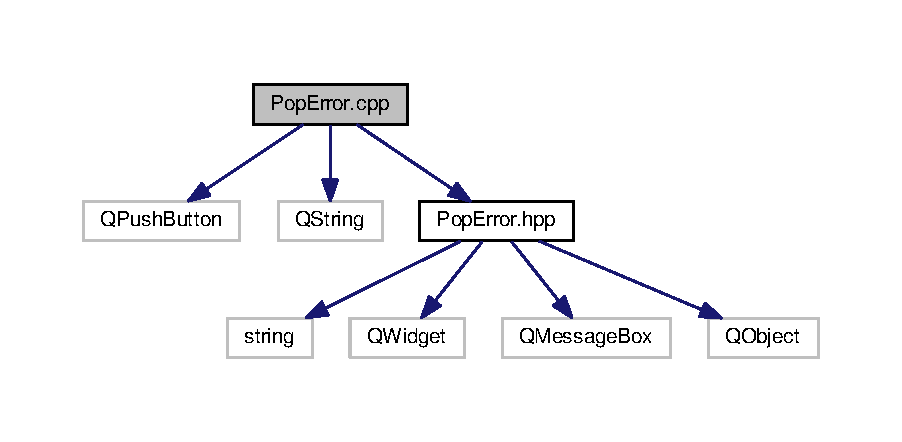
\includegraphics[width=350pt]{PopError_8cpp__incl}
\end{center}
\end{figure}

\hypertarget{PopError_8hpp}{}\section{gui/\+Pop\+Error.hpp File Reference}
\label{PopError_8hpp}\index{gui/\+Pop\+Error.\+hpp@{gui/\+Pop\+Error.\+hpp}}


....  


{\ttfamily \#include $<$string$>$}\\*
{\ttfamily \#include $<$Q\+Widget$>$}\\*
{\ttfamily \#include $<$Q\+Message\+Box$>$}\\*
{\ttfamily \#include $<$Q\+Object$>$}\\*
Include dependency graph for Pop\+Error.\+hpp\+:
% FIG 0
\subsection*{Classes}
\begin{DoxyCompactItemize}
\item 
class \hyperlink{classPopError}{Pop\+Error}
\begin{DoxyCompactList}\small\item\em .... \end{DoxyCompactList}\end{DoxyCompactItemize}


\subsection{Detailed Description}
.... 

\begin{DoxyAuthor}{Author}
G\+RI Team 
\end{DoxyAuthor}
\begin{DoxyDate}{Date}
06/23/2017 
\end{DoxyDate}
\begin{DoxyVersion}{Version}
1.\+0 
\end{DoxyVersion}

\hypertarget{RegistrationWindow_8cpp}{}\section{Registration\+Window.\+cpp File Reference}
\label{RegistrationWindow_8cpp}\index{Registration\+Window.\+cpp@{Registration\+Window.\+cpp}}
{\ttfamily \#include $<$Q\+Main\+Window$>$}\\*
{\ttfamily \#include $<$Q\+Push\+Button$>$}\\*
{\ttfamily \#include $<$Q\+Line\+Edit$>$}\\*
{\ttfamily \#include $<$Q\+Status\+Bar$>$}\\*
{\ttfamily \#include $<$Q\+Label$>$}\\*
{\ttfamily \#include $<$Q\+Color$>$}\\*
{\ttfamily \#include $<$Q\+Palette$>$}\\*
{\ttfamily \#include $<$Q\+Pixmap$>$}\\*
{\ttfamily \#include $<$Q\+Object$>$}\\*
{\ttfamily \#include $<$Q\+Size$>$}\\*
{\ttfamily \#include $<$Q\+Icon$>$}\\*
{\ttfamily \#include $<$iostream$>$}\\*
{\ttfamily \#include $<$Q\+Tool\+Tip$>$}\\*
{\ttfamily \#include $<$Q\+Application$>$}\\*
{\ttfamily \#include \char`\"{}Registration\+Window.\+hpp\char`\"{}}\\*
{\ttfamily \#include \char`\"{}../core/\+Validation\+Info.\+hpp\char`\"{}}\\*
Include dependency graph for Registration\+Window.\+cpp\+:
\nopagebreak
\begin{figure}[H]
\begin{center}
\leavevmode
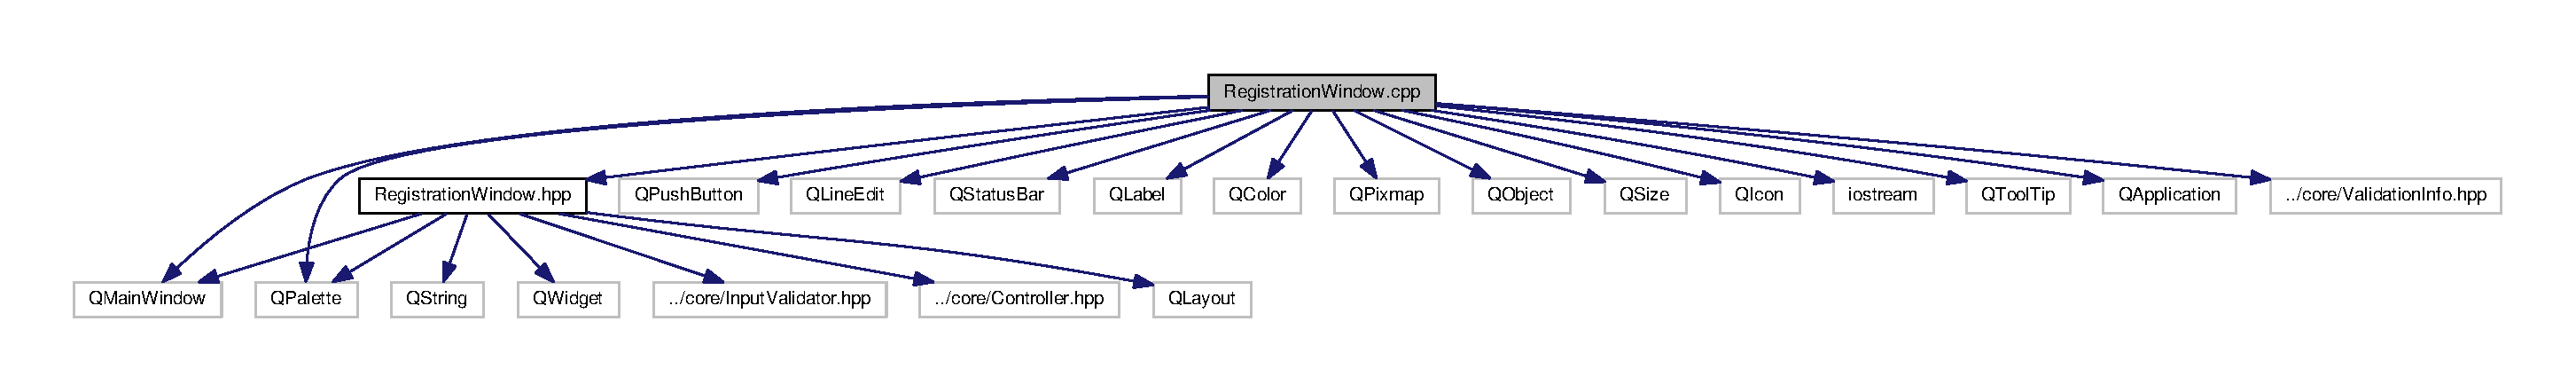
\includegraphics[width=350pt]{RegistrationWindow_8cpp__incl}
\end{center}
\end{figure}

\hypertarget{RegistrationWindow_8hpp}{}\section{gui/\+Registration\+Window.hpp File Reference}
\label{RegistrationWindow_8hpp}\index{gui/\+Registration\+Window.\+hpp@{gui/\+Registration\+Window.\+hpp}}


\hyperlink{RegistrationWindow_8hpp}{Registration\+Window.\+hpp} creating a G\+UI for registration window and connection for checking params for registration.  


{\ttfamily \#include $<$Q\+Main\+Window$>$}\\*
{\ttfamily \#include $<$Q\+Layout$>$}\\*
{\ttfamily \#include $<$Q\+String$>$}\\*
{\ttfamily \#include $<$Q\+Palette$>$}\\*
{\ttfamily \#include $<$Q\+Widget$>$}\\*
{\ttfamily \#include \char`\"{}../core/\+Input\+Validator.\+hpp\char`\"{}}\\*
{\ttfamily \#include \char`\"{}../core/\+Controller.\+hpp\char`\"{}}\\*
Include dependency graph for Registration\+Window.\+hpp\+:
% FIG 0
This graph shows which files directly or indirectly include this file\+:
% FIG 1
\subsection*{Classes}
\begin{DoxyCompactItemize}
\item 
class \hyperlink{classRegistrationWindow}{Registration\+Window}
\begin{DoxyCompactList}\small\item\em \hyperlink{classRegistrationWindow}{Registration\+Window} class which creates the G\+UI for login window. \end{DoxyCompactList}\end{DoxyCompactItemize}


\subsection{Detailed Description}
\hyperlink{RegistrationWindow_8hpp}{Registration\+Window.\+hpp} creating a G\+UI for registration window and connection for checking params for registration. 

\begin{DoxyAuthor}{Author}
G\+RI Team 
\end{DoxyAuthor}
\begin{DoxyDate}{Date}
06/14/2017 
\end{DoxyDate}
\begin{DoxyVersion}{Version}
1.\+0 
\end{DoxyVersion}

%--- End generated contents ---

% Index
\backmatter
\newpage
\phantomsection
\clearemptydoublepage
\addcontentsline{toc}{chapter}{Index}
\printindex

\end{document}
